\documentclass[12pt,a4paper,titlepage]{article}
\usepackage[utf8]{inputenc}
\usepackage[russian]{babel}
\usepackage[OT1]{fontenc}
\usepackage{amsmath}
\usepackage{amsfonts}
\usepackage{amssymb}
\usepackage{graphicx}
\author{Н.Е.Богданов}
\title{ « Параллельные вычисления »}
\frenchspacing
\begin{document}
\maketitle
\tableofcontents
\newpage
\section{Задание}

\begin{enumerate}
\item 
Постановка задачи
\begin{itemize}
\item 
Описание назначения проектируемой системы
\item 
Функциональные требования (текстовое описание Участников и их Интересов)
\item
Описание бизнес-процессов (этапы, Участники)
\end{itemize} 
\item
Разработка вариантов использования (обобщенная диаграмма(ы) прецедентов для всех ролей)
\item
Подробное описание всех вариантов использования (текстовое описание с альтернативами)
\item
Разработка статической объектной модели предметной области (диаграмма классов)
\item
Разработка динамической объектной модели предметной области (диаграмма последовательности)
\item
Проектирование слоя бизнес-логики (выбор архитектурного шаблона уровня бизнес-логики)
\item
Реализация слоя бизнес-логики (Java, NetBeans), unit-тестирование (JUnit), вместо слоя хранения - шаблон "Репозиторий"
\item
Проектирование слоя источников данных (выбор архитектурного шаблона уровня доступа к данным: DB + внешний сервис)
\item
Реализация слоя источников данных (JavaDB, NetBeans), unit-тестирование
\item
Проектирование сервисного слоя и слоя представления: GUI (Swing), внешний сервис
\item
Реализация слоев представления, сервисного слоя, unit-тестирование сервисного слоя
\item
Комплексное тестирование системы
\item
Пояснительная записка (включает все разделы, указанные выше, а также выводы)
\end{enumerate}
\section{Решение}
\subsection{Постановка задачи}
Заказ услуг по строительным работам.
Создание и управления заказами на строительные работы, а так же учёт требуемых ресурсов на складе.
\subsection{Роли}
\begin{itemize}
\item Клиент
\begin{enumerate}
\item Заказывает работу.
\item Принимает результат.
\item Оплачивает работу.
\end{enumerate}
\item Менеджер
\begin{enumerate}
\item Составляет смету + смету доработок (на основе списка доработок от Прораба).
\item Ведёт учёт ресурсов со склада.(дозаказывает по мере надобности).
\item Ведёт учёт бюджета компании.
\item Принимает оплату от клиента.
\end{enumerate}
\item Прораб
\begin{enumerate}
\item Получает список работ.
\item Выполняет работу.
\item Составляет список доработок.
\item Отдаёт работу на приём Клиенту.
\end{enumerate}
\end{itemize}
\newpage
\subsection{Подробное описание вариантов использования}
\begin{enumerate}
\item
Процесс оформления заказа. прописываются все требуемые ресурсы и услуги оказываемые прорабом. Если ресурсов на складе не хватает то происходит дополнительный заказ ресурсов.
\item
Процесс сдачи/приёма работы.

2 Варианта:
\begin{itemize}
\item Первый. Успешная сдача объекта клиент принимает работу прораба и получает смету (составленную менеджером) со списком проведённых работ.
\item Второй. В случае если клиент требует доработки, прораб составляет список требуемых работ и(или) ресурсов), а менеджер составляет смету доработок,после чего клиент оплачивает 85\% от текущего заказа без сметы доработок. а дальше выполняются действия как в первом варианте или повторные доработки.
\end{itemize}
\item
Процесс оплаты счёта. 2 варианта действий, клиент может оплатить:
	\begin{itemize}
		\item наличными или
		\item по безналичному расчёту.
	\end{itemize}
\end{enumerate}
\newpage
\subsection{Use - case диаграмма}
\begin{figure}[!ht]
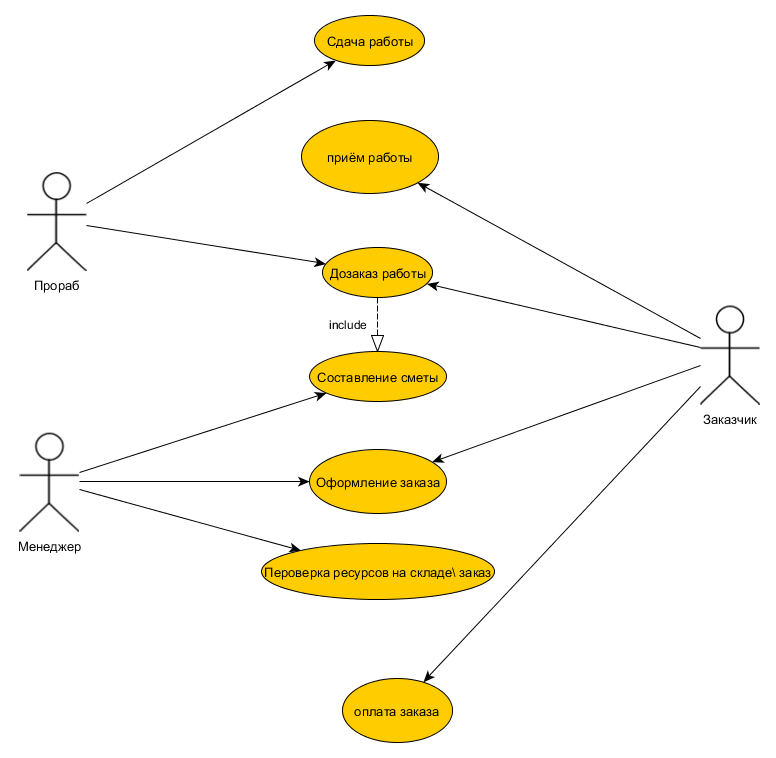
\includegraphics[scale=0.5]{uml_use_case.png}\caption{}
\end{figure}
\newpage
\subsection{Статическая модель предметной области (uml диаграмма классов)} 
\begin{figure}[!ht]
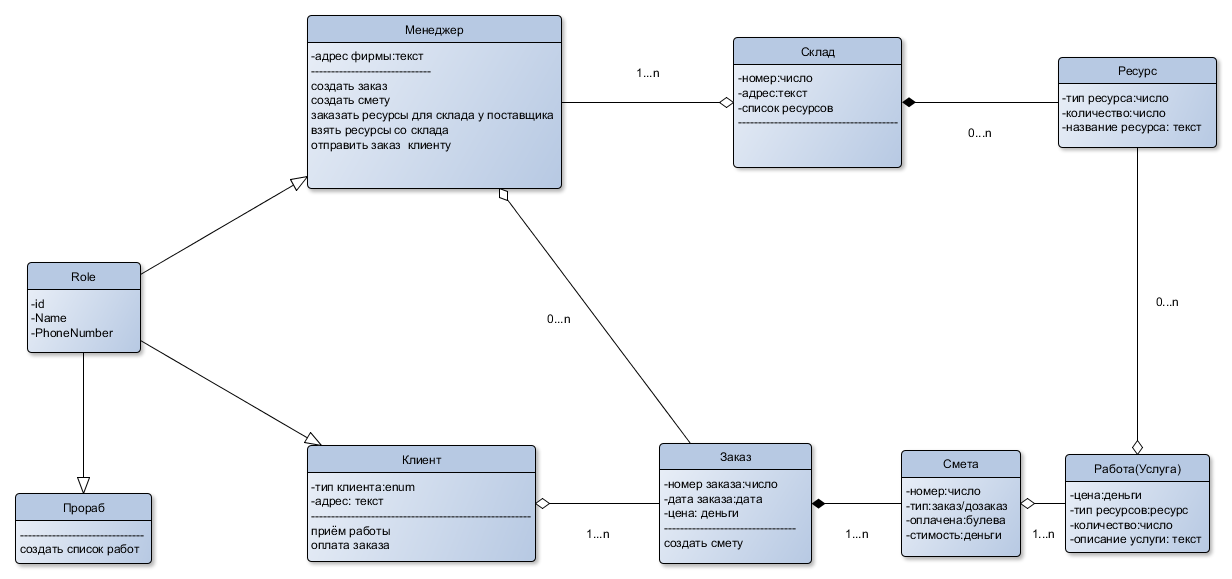
\includegraphics[scale=0.3]{uml_class_diagram.png}\caption{}
\end{figure}
\newpage
\subsection{Диаграмма последовательностей}
\begin{figure}[!ht]
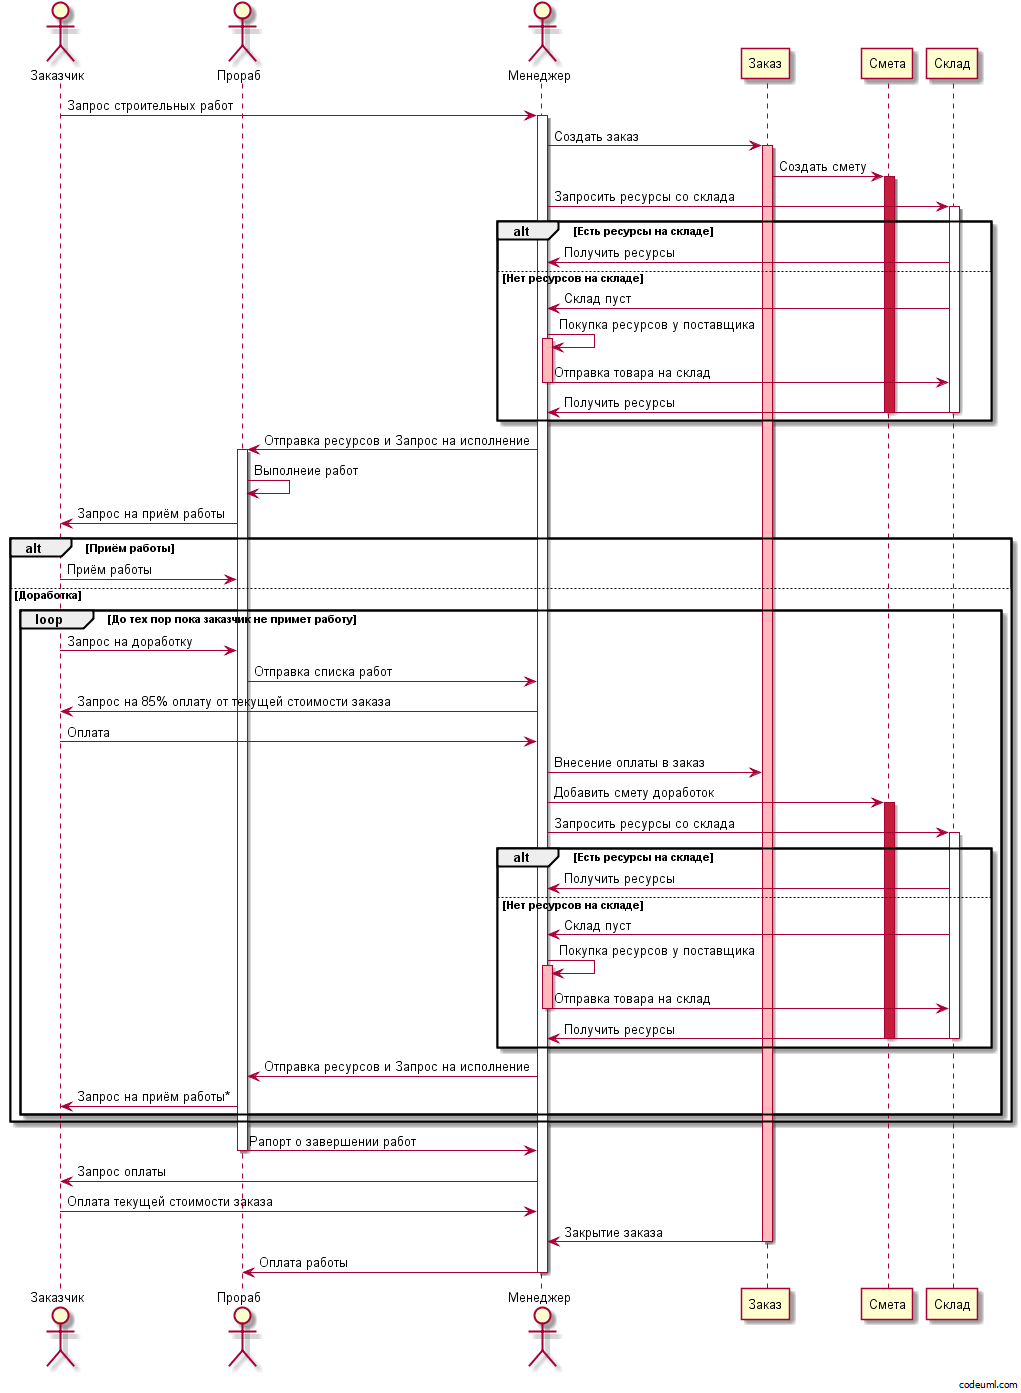
\includegraphics[scale=0.5]{getimage.png}\caption{}
\end{figure}
\newpage
\subsection{Слой бизнес-логики}
\newpage
\subsection{Слой источников данных}
\newpage
\subsection{Сервисный слой и слой представления}
\newpage
\section{Тестирование}
\newpage
\section{Заключение}
\end{document}